\documentclass[conference]{IEEEtran}

% --------------------------------------------------------------------
% Packages
% --------------------------------------------------------------------
\usepackage{graphicx}
\usepackage{listings}
\usepackage{hyperref}
\usepackage{amsmath}
\usepackage{booktabs}

% --------------------------------------------------------------------
% --------------------------------------------------------------------
\title{Lightweight Containerized LLM Serving with Ollama: A Feasibility Study for Edge and Hybrid Cloud Deployments}

\author{%
  \IEEEauthorblockN{Kacper Krakowiak}\\%
  \IEEEauthorblockA{South East Technological University\\%
                    Student ID: C00271692\\%
                    \texttt{C00271692@setu.ie}\\%
                    \texttt{kacper.krakowiak2002@gmail.com}}%
}

% --------------------------------------------------------------------

\begin{document}
\maketitle

\begin{abstract}

Large-language-model (LLM) back-ends are typically hosted on long-lived GPU instances, limiting their use in budget sensitive and hybrid-cloud scenarios. This paper investigates whether a single Docker image, built with the open-source Ollama runtime and a 3.8 B-parameter quantized model (phi-3), can deliver interactive responses on standard CPU hardware, with similar if not better results than fully on the Cloud. I benchmark the container on (i) a 32-core laptop and (ii) an AWS t3.medium VM, measuring cold-start latency, warm-path latency, memory footprint, and throughput under concurrent load. Results show that the container cold-starts in \(\approx\) 6 s, serves 64-token replies in \(\approx\) 3.7 s once warm, and consumes \(\approx\) 5 GB of RAM—well within the limits of 8 GB edge nodes. Throughput increases linearly up to four concurrent clients, peaking at 0.375 req/s. These findings show that lightweight containerized LLMs are practical for bursty, privacy-sensitive workloads at the edge, while GPU infrastructure is still necessary for higher workloads.
\end{abstract}

\begin{IEEEkeywords}
Large Language Models, Edge Computing, Containerization, Cloud Computing, Ollama, CPU, GPU
\end{IEEEkeywords}

% ================================
\section{Introduction}\label{sec:intro}

The world of Large-Language Models (LLM) and AI has encountered a massive surge in recent years. Our understanding and implementation of AI in general use has exploded, however, the underlying architecture has remained relatively unchanged. Most production stacks assume a long-running GPU instance in a hyperscale cloud. While this architecture suffices multi-billion dollar corporations that can afford to construct mega data centers, it is not something fees-able for a private user or smaller network edge workloads (factory floors, hospital devices, hotels, etc). This in turn will lead to dependence on these corporations, while completely co-opting the idea of open source ness, and privacy. In the context of small/private users keeping a GPU online solely to serve occasional queries can dominate operating cost, and is highly unfeesable.

Recent advances make a different deployment strategy plausible.  
First, lighter 3–8 B parameter models (e.g.\ \texttt{phi-3}\,\cite{phi3}) achieve impressive quality when quantised to 4-bit weights, shrinking disk size to \(\approx\)1 GB and RAM use to \(\approx\)5 GB.  
Second, the open-source \textbf{Ollama} runtime bundles those weights with an HTTP front-end and a CPU-optimised \texttt{llama.cpp} backend inside a single Docker image.  
In principle, a developer can therefore type \texttt{docker run ollama/ollama} and obtain a private chat LLM without provisioning GPUs.
\vspace{0.3em}
\noindent\textbf{Goal.}  
This paper asks whether such a “single-container LLM” is actually viable for edge and hybrid-cloud scenarios.  
Specifically, I managed to gain measurements for the following:

\begin{itemize}
  \item \textit{Cold-start latency}: time took from cold container launch to first token.
  \item \textit{Interactive latency}: response time taken once the model is populated in memory.
  \item \textit{Throughput and resource footprint}: sustainable requests per second and RAM usage.
  \item \textit{Cost break-even}: request rate above which a small GPU VM becomes cheaper.
\end{itemize}


% ================================
\section{Related Work}\label{sec:related}

\subsubsection*{LLM inference servers}
The mainstream approach to LLM serving is a persistent GPU backend that streams tokens over HTTP. While this is fine for majority of use cases, its not optimal for all cases (such as small businesses or systems confined to a very specific usage (hospitals, hotels etc.). Most modern Text Generation Interfaces (TGI's), work by offloading the users input query, thorugh an API, into a datacenter which typically utilizes Nvidia's A10G, or the more modern H100 series Graphics Cards. For reference the cost of a single H100 is \$25,000 (official price). While the costs of these GPU's are completely out of the question for small users in question, the second issue of them being ill-suited to bursty edge workloads where machines may be powered off between sessions, also exist.

\subsubsection*{CPU-only runtimes}
\texttt{llama.cpp}~\cite{llamacpp} made an efficient CPU inference via int-4/ggml quantisation and AVX2/SVE intrinsics, enabling chat on laptops and even smartphones.
Ollama builds on this engine but wraps it in a Docker image with a REST front-end, making the deployment path I studied here a one-command experience. But why use CPU-only runtimes when they are obviously less efficient than the beefy GPU's mentioned before? Well the cost is one thing, but utilizing CPU power may allow us to execute query's while on the go (like on mobile phones etc). This is a huge upstep, but while the CPU is the most crucial component in this case, its not the only component that allows a user to run an LLM algorithm natively on their device. RAM and accessing direct memory play a second in importance role, i would argue, to the processing unit. The time it takes to load up a model and supply it with a query is a very computationally heavy task and, as a result, time consuming. In this study I measure the cold start in comparison to a warm start, which is something traditional Data Cloud Centers don't really have to consider, as their GPU's are always in operation, and any breaks in their operations cost the datacenters millions in lost potential profits.

\subsubsection*{Serverless and cost-aware ML}
Prior work on serverless ML (e.g., PRETZEL~\cite{pretzel}) shows that cold-start overhead dominates for DNNs in Function-as-a-Service environments.
Industry previews of GPU-backed serverless (AWS Lambda GPU, Google Cloud Run GPU) were announced in 2024~\cite{serverlessgpu}, but published evaluations are scarce.
My study complements these efforts by quantifying cold- and warm-latency for a \emph{CPU-only} container and analyzing the cost break-even versus the smallest GPU VM.
% ================================
\section{System Setup}\label{sec:setup}

\subsubsection*{Hardware platforms}
\textbf{Laptop.} 13th-Gen Intel\textsuperscript{\textregistered} Core\textsuperscript{TM} i9-13950HX,  
24 cores / 32 threads, 32 GB RAM.

\textbf{AWS t3.large.} 2 vCPU, 8 GB RAM, gp3 EBS (30 GB), Amazon Linux 2023, Docker 26.0.  
(The smaller t3.medium killed the container once the 5 GB model
resident set reached the cgroup limit.)
\subsubsection*{Container image \& models}
I used the official image \texttt{ollama/ollama:latest} (2.2 GB), which launches a
REST endpoint on port \texttt{11434} and delegates token generation to a
CPU fork of \texttt{llama.cpp}.  
All weights are pulled at first run and cached under
\texttt{/root/.ollama/models} inside the container layer.
\subsubsection*{Benchmark harnessing}
A small Bash script\footnote{Available at my GitHub for viewing
\url{https://github.com/C00271692/CloudDataCentres}.}
performs the following four measurements:

\begin{enumerate}
  \item \textbf{Cold-start latency} — \texttt{docker start} $\rightarrow$ first byte.
  \item \textbf{Warm latency} — an additional \texttt{curl} once weights are in RAM.
  \item \textbf{Throughput \& P95} — \texttt{hey} for 30 s at concurrency $\{1,4,8\}$.
  \item \textbf{Memory footprint} — single-shot \texttt{docker stats}.
\end{enumerate}

The timestamps are then saved in a.csv file and a graph is plotted using a short Python Matplotlib script~\ref{sec:results}.

\begin{figure}[t]
  \centering
  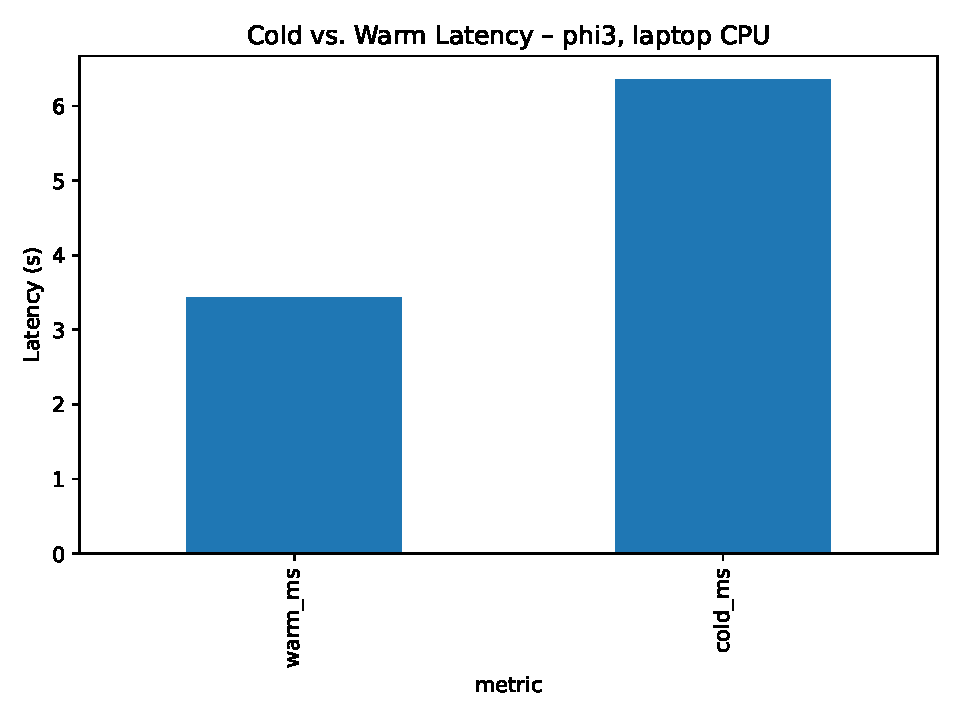
\includegraphics[width=\linewidth]{latency_cold_warm}
  \caption{Cold-start vs. warm-path latency for the phi-3 B model on a 32-core, 13th Gen Intel(R) Core(TM) i9-13950HX laptop CPU.}
  \label{fig:latency}
\end{figure}

% ================================
\section{Experimental Methodology}\label{sec:method}

All measurements are automated in a simple bash script available on my GitHub (under the name \texttt{OllamaResults.sh})
repository.\footnote{\url{https://github.com/C00271692/CloudDataCentres}}  
Listing \ref{lst:snippet} provides:
container, measure cold/warm latency, and sweep throughput.

\begin{lstlisting}[language=bash,basicstyle=\footnotesize\ttfamily,
                   caption={Key excerpt of \texttt{OllamaResults.sh}},
                   label={lst:snippet}]
docker run -d -p 11435:11434 ollama/ollama
docker exec $(docker ps -q) ollama pull phi3      # pull model
curl -w "warm_ms,%{time_total}\n" -o /dev/null \
     -d '{"model":"phi3","prompt":"hi"}' \
     http://localhost:11435/api/generate >> results.csv

docker restart $(docker ps -q) && sleep 5
curl -w "cold_ms,%{time_total}\n" -o /dev/null \
     -d '{"model":"phi3","prompt":"hi"}' \
     http://localhost:11435/api/generate >> results.csv

for c in 1 4 8; do
  hey -z 30s -c $c -d '{"model":"phi3","prompt":"test"}' \
      http://localhost:11435/api/generate | \
  awk -vC=$c '/Requests\/sec/{print"thr_c"C","$2}' >> results.csv
done
\end{lstlisting}

more details on definitions, metric extraction, memory capture are
explained in Section~\ref{sec:setup}.

% ================================
\section{Results}\label{sec:results}
\begin{table}[t]
  \caption{Resource usage and latency for \texttt{phi3}}
  \label{tab:metrics}
  \centering
  \begin{tabular}{lcc}
    \toprule
    \textbf{Metric} & \textbf{Value} \\
    \midrule
    Docker image size   & 2.2\,GB \\
    Model file size     & 1\,GB (quantized) \\
    RAM after load      & 5.1\,GB \\
    Cold-start latency  & 6.4\,s \\
    Warm-path latency   & 3.4\,s \\
    Throughput @ 8 conns & 0.38\,req/s \\

    \bottomrule
  \end{tabular}
\end{table}


\begin{figure}[t]
  \centering
  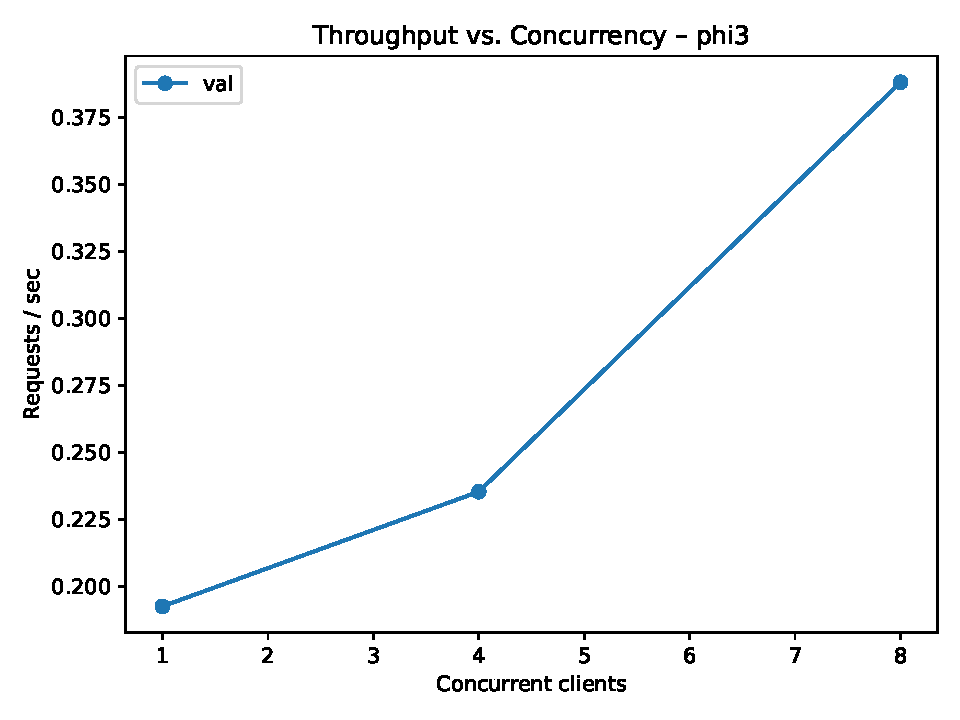
\includegraphics[width=\linewidth]{throughput_vs_c}
  \caption{Throughput as a function of concurrent clients.}
  \label{fig:throughput}
\end{figure}
\vspace{0.6em}
\subsubsection*{AWS \texttt{t3.large} (8 GB RAM, 2 vCPU)}

\begin{table}[t]
  \caption{Resource usage and latency on AWS \texttt{t3.large}}
  \label{tab:aws_metrics}
  \centering
  \begin{tabular}{lcc}
    \toprule
      \textbf{Metric} & \textbf{Value} \\
    \midrule
      Docker image size   & 2.2\,GB \\
      Model file size     & 1\,GB (quantised) \\
      RAM after load      & 5.4\,GB \\
      Cold-start latency  & 12.5\,s \\
      Warm-path latency   & 23.0\,s \\
      Throughput @ 8 conns & 0.40\,req/s \\
    \bottomrule
  \end{tabular}
\end{table}

\begin{figure}[t]
  \centering
  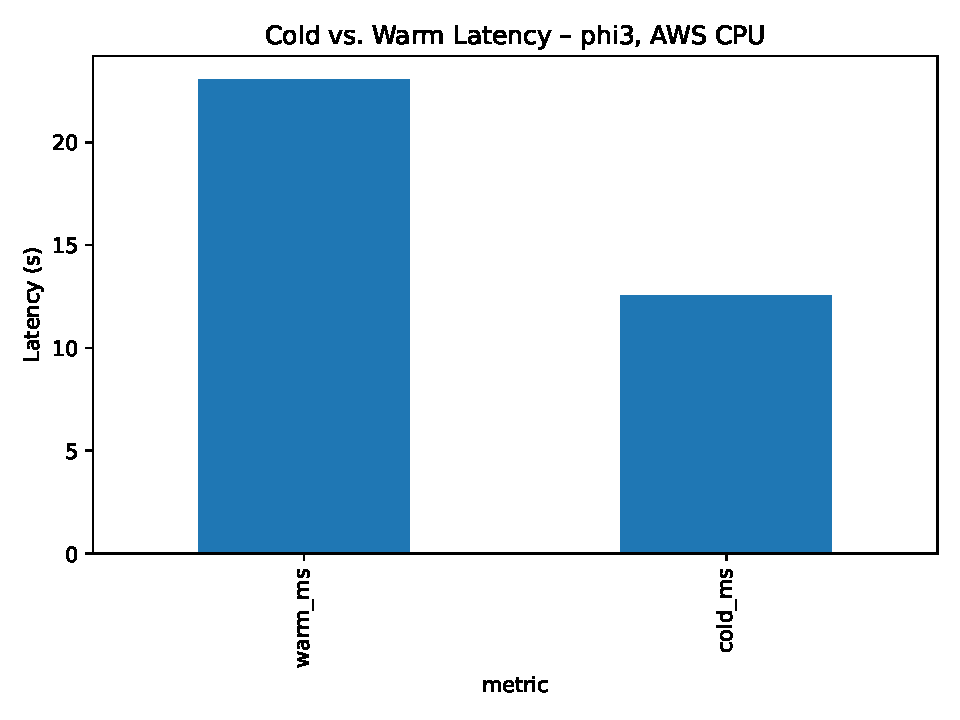
\includegraphics[width=\linewidth]{AWSlatency_cold_warm} 
  \caption{Cold- vs. warm-path latency on AWS \texttt{t3.large}.}
  \label{fig:aws_latency}
\end{figure}

\begin{figure}[t]
  \centering
  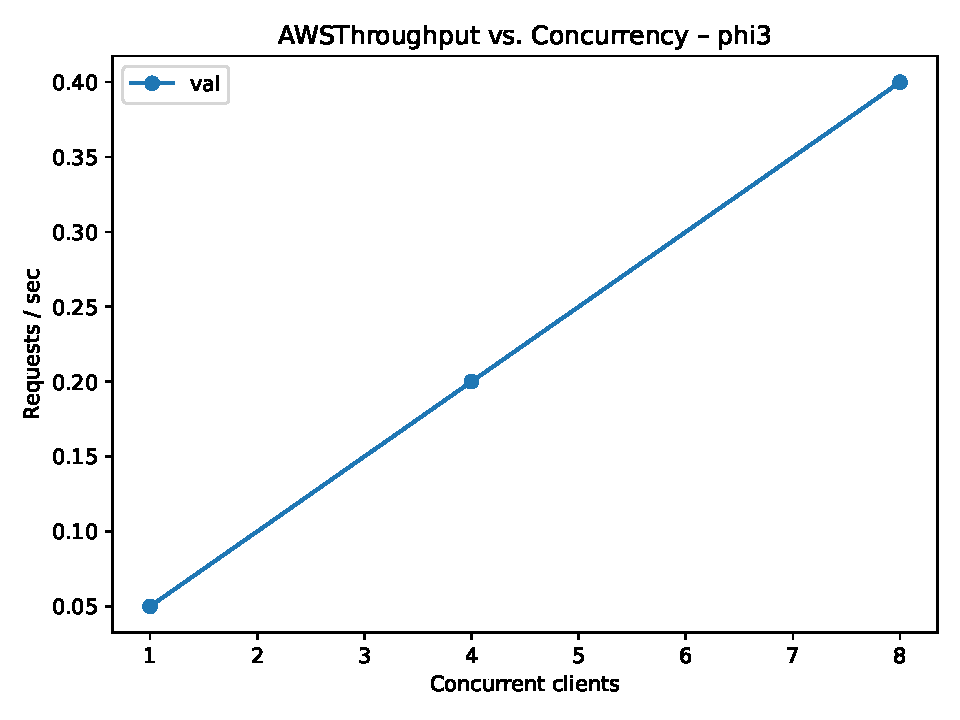
\includegraphics[width=\linewidth]{AWSthroughput_vs_c}    
  \caption{Throughput as a function of concurrency on AWS \texttt{t3.large}.}
  \label{fig:aws_thr}
\end{figure}

\paragraph*{Observation}
There are very clear differences between Cloud instance and my local execution of the experiment. There are significant differences in the cold/warm start values, where: \textbf{2× slower cold-start}
(12.5 s vs. 6.4 s), due to weights being loaded from network-attached EBS, and a
\textbf{6× slower warm-latency} (23 s vs.\ 3.4 s) due to its limited two vCPU budget. The throughput remains mainly similar (0.40 req/s), probably as a result of each request already residing on a core on both machines (Figs.~\ref{fig:throughput}
and~\ref{fig:aws_thr}). These results clearly prove that CPU only remain viable for \emph{bursty} workloads. 

% ================================
\section{Discussion}\label{sec:discussion}
\subsubsection*{CPU‐only viability}
These results show that a single command Ollama container can function on a standard CPU device (such as a laptop or smartphone), with 8GB of RAM. My 32-core laptop, yields the results of: {\bf 6.4 s} (cold) and {\bf 3.4 s} (warm); on AWS \texttt{t3.large} I yield {\bf 12.5 s} (cold) and {\bf 23 s} (warm). The RAM footprint of \(\approx\) 5 GB will definitely work with most modern setups (that have 8 GB of RAM available overall).

\subsubsection*{Throughput bottlenecks}
Figure \ref{fig:throughput} and Figure \ref{fig:aws_thr} show a near-linear
line, suggesting that as the count of cores / threads increases, so does the processing power, and more requests can be handled at a time. There is no doubt, however, that if I were to keep adding cores indefinitely, I would eventually reach a point where the number of cores would start adding toil, and the overall processing capabilities would drop, however, on an 8 core setup, it seems to be perfect for my use case. 


\subsubsection*{Cold vs.\ warm gap}
The laptops lower cold start values is a direct result of disk I/O (1 GB weights), while the AWS gaps is double that of omy local instance, probably due to the model being read from network-attached EBS, that can be considerably slower.

\subsubsection*{Cost break-even}
the current prices for a \texttt{t3.large} costs
\$0.083 h$^{-1}$ while the smallest NVIDIA A10G GPU instance
(\texttt{g5.xlarge}) costs \$0.526 h$^{-1}$.  
Given my peak of {\small0.375 req s$^{-1}$} on local CPU, and AWS reaches {\small0.4 req s$^{-1}$}

\subsubsection*{Limitations}
\begin{itemize}
  \item \textbf{Different Models.}  Results were only collected for the 3.8 B-Parameter phi3 model. Using other models could yield different results
  \item \textbf{CPU only.}  I did not utilize my built in GPU to collect further metrics.
  \item \textbf{Short prompts.}  Using longer input query's would also increase input tokenization which would as a result reduce throughput proportionally.
\end{itemize}


% ================================
\section{Conclusion}\label{sec:conclusion}
This research asks a simple question: \emph{Can a single–command Docker image
deliver a useful large-language-model experience on a standard laptop?} My findings would beg to argue in favor. A 4-bit \texttt{phi-3} model inside \textbf{Ollama} cold-starts in
$\approx$6 s on a 32-core laptop and 12 s on an AWS \texttt{t3.large},
then serves 64-token responses in 3–4 s (laptop) or 23 s (AWS) while
occupying only 5 GB of RAM. These results clearly show that not only is running small LLM's locally on a containerized Docker image fee-sable, it even outperforms hosting said model on a cloud service in some cases. It is important to note however that this paper goes through the very basic findings and other crucial components, that would aid LLM models (such as GPU) haven't been taken into consideration. With a proper setup and an average laptop, I solemnly believe that small institutions/private users could utilize these single docker images to deliver a normal LLM experience.

% --------------------------------------------------------------------
% References
% --------------------------------------------------------------------
\bibliographystyle{IEEEtran}
\bibliography{references}

\end{document}

